\documentclass[11pt]{article}

\usepackage{ifpdf}
\usepackage{ifxetex}
\usepackage{color}
\usepackage{amsmath}
\usepackage{amsfonts}
\usepackage{booktabs}
\usepackage{tabularx}
\usepackage{colortbl}
\usepackage{multirow}
\usepackage{xcolor}
\usepackage{subfigure}
\usepackage{dcolumn}
\usepackage{flushend}
\usepackage{capt-of}
\usepackage[T1]{fontenc}
\usepackage{libertine}
\renewcommand*\oldstylenums[1]{{\fontfamily{fxlj}\selectfont #1}}
\usepackage{tikz}
\usetikzlibrary{positioning}
\usepackage{arydshln}
\usepackage{booktabs}
\usepackage{rotating}
% \usepackage{hyperref}
\usepackage{graphicx}
\DeclareGraphicsExtensions{.pdf,.eps,.png,.jpg}
\graphicspath{{./figures/}}

% for code listings
\usepackage{listings}

% correct bad hyphenation here
\hyphenation{op-tical net-works semi-conduc-tor}

\newcommand{\DATE}{\today} \newcommand{\LTYPE}{latex2e}
\newcommand{\reffig}[1]{Fig.~\ref{fig:#1}}
\newcommand{\reftab}[1]{Table~\ref{tab:#1}}
\newcommand{\refsec}[1]{Section~\ref{sec:#1}}
\newcommand{\refchap}[1]{Chapter~\ref{chap:#1}}
\newcommand{\reflem}[1]{Lemma~\ref{lem:#1}}
\newcommand{\refthm}[1]{Theorem~\ref{thm:#1}}
\newcommand{\refeq}[1]{Equation~(\ref{eq:#1})}
\newcommand{\ceil}[1]{\left\lceil #1 \right\rceil}
\newcommand{\floor}[1]{\lfloor #1 \rfloor}

\definecolor{Navy}{rgb}{0.1,0.1,0.41}
\definecolor{linkcol}   {named}{Navy}
\definecolor{citecol}   {rgb}{.5,0,0}
\definecolor{urlcol}    {rgb}{0,0,1}

\newcommand{\QTWO}{\emph{$Q^2$}}
\newcommand{\Quipu}{\emph{Quipu}}
\newcommand{\QUAD}{{\sc Quad}}
\newcommand{\MAIP}{{\sc Maip}}
\newcommand{\gprof}{\emph{gprof}}
\newcommand{\DWB}{\emph{DWB}}
\newcommand{\DelftWorkbench}{\emph{Delft Workbench}}
\newcommand{\DWARV}{\emph{DWARV}}
\newcommand{\TIMES}{$\times$}
\newcommand{\MCPROF}{\emph{MCProf}}

%-----------------------------------------------------------------------------------------
\begin{document}

% paper title
\title{\MCPROF{}: Memory and Communication Profiler}
\author{Imran Ashraf \\
    Computer Science and Engineering\\
    Department of Software and Computer Technology\\
    Delft University of Technology, Delft, The Netherlands\\
    I.Ashraf@tudelft.nl
}
\maketitle

%----------------------------------------------------------------------------------
\section{Introduction}
\label{sec:introduction}

\MCPROF{} is a memory and communication profiler. It traces memory reads/writes and reports
memory accesses by various functions in the application as well as the
data-communication between functions. The information is obtained by
performing dynamic binary instrumentation by utilizing Intel Pin \cite{Pin} framework.
This manual explains the process of setting up \MCPROF{} and using it.



%----------------------------------------------------------------------------------
\section{Availability}
\label{sec:availability}

\MCPROF{} can be downloaded from ...


%----------------------------------------------------------------------------------
\section{Required Packages}
\label{sec:reqPackages}

In order to setup and use \MCPROF{} the following two packages are required:

\begin{itemize}
\item Intel Pin DBI framework \cite{Pin} Revision 62732 or higher
\item g++ compiler with support for C++11X
\item  graphviz Dot utility for converting the generated communication graphs from DOT to pdf formats
\end{itemize}


%----------------------------------------------------------------------------------
\section{Installation}
\label{sec:installation}

\MCPROF{} uses Makefile to compile the sources. In order to compile \MCPROF{} from
sources on 32-bit / 64-bit Linux, the following steps can be performed.

\begin{itemize}

\item Download Pin and copy and extract it to the directory where you want to keep Pin.

\item Define a variable \verb|PIN_ROOT| by running the following commands:
        \begin{center}
        \verb|export PIN_ROOT=/<absolute path to pin>|
        \end{center}

\item You can also add this line, for instance, to your \textbf{.bashrc} in case you are
using \textbf{bash} to export the variable automatically on opening a terminal.

\item Download \MCPROF{} and copy and extract it to the directory where you want to compile it.

\item Go the \MCPROF{} directory and run the following command to compile:
        \begin{center}
        \verb|make|
        \end{center}

\end{itemize}

If every thing goes fine, you will see a directory \verb|obj-intel64| (or \verb|obj-ia32|
depending upon your architecture). This directory will contain the executables and
object files generated as a result of the compilation. The important files are:

\begin{itemize}
\item \textbf{mcprof.so} which is the tool. This will be used to profile the
applications as explained in Section \ref{sec:usage}.
\item executable files of the test applications available in \textbf{tests} directory.
These executables can be used as test inputs.
\end{itemize}



%----------------------------------------------------------------------------------
\section{Usage}
\label{sec:usage}

In order to explain the usage of \MCPROF{} we will use the example application
listed in Figure \ref{fig:vectOps}. The source code is available in \verb|tests|
directory of source package.

\begin{figure} %[ht]
    \centering
%     \lstinputlisting[basicstyle=\scriptsize,language=C,showstringspaces=false,frame=bt]{code/example.c}
    \lstinputlisting
    [
    language=C,
    showstringspaces=false,
    frame=bt,
    numbers=left,
    stepnumber=1,
    basicstyle=\small %\tiny
    ] {code/vectOps.c}
    \caption{Example of an application processing some arrays.}
    \label{fig:vectOps}
\end{figure}


\subsection{Using Given Tests}

This example will be compiled during the default compilation of the
\MCPROF{} discussed in Section \ref{sec:installation}. In order to profile this
application by \MCPROF{} you can give the following command:
        \begin{center}
        \verb|make vectOps.test|
        \end{center}

Simmilarly, other tests can also be executed by replacing the <vectOps> with the
<name of the test application>.test as given in \textbf{tests} directory. This
will generate the output information depending upon which engines is used. This
will be explained in Section \ref{sec:output}.

\subsection{Using Your Own Example}

This application can be compiled 


%----------------------------------------------------------------------------------
\section{Output}
\label{sec:output}



%----------------------------------------------------------------------------------
\section{Contact}
\label{sec:contact}

In case you are interested in contributing to \MCPROF{}, or you have suggestions for
improvements, or you want to report a bug, contact:

\begin{itemize}
\item Imran Ashraf < I.Ashraf@TUDelft.nl >
\end{itemize}

%----------------------------------------------------------------------------------
% references section
\bibliographystyle{unsrt}
\bibliography{bib/references}

% that's all folks
\end{document}
%----------------------------------------------------------------------------------



% an example of a figure \ref{fig:figure1}.
% \begin{figure}[!bt]
% \centering
% 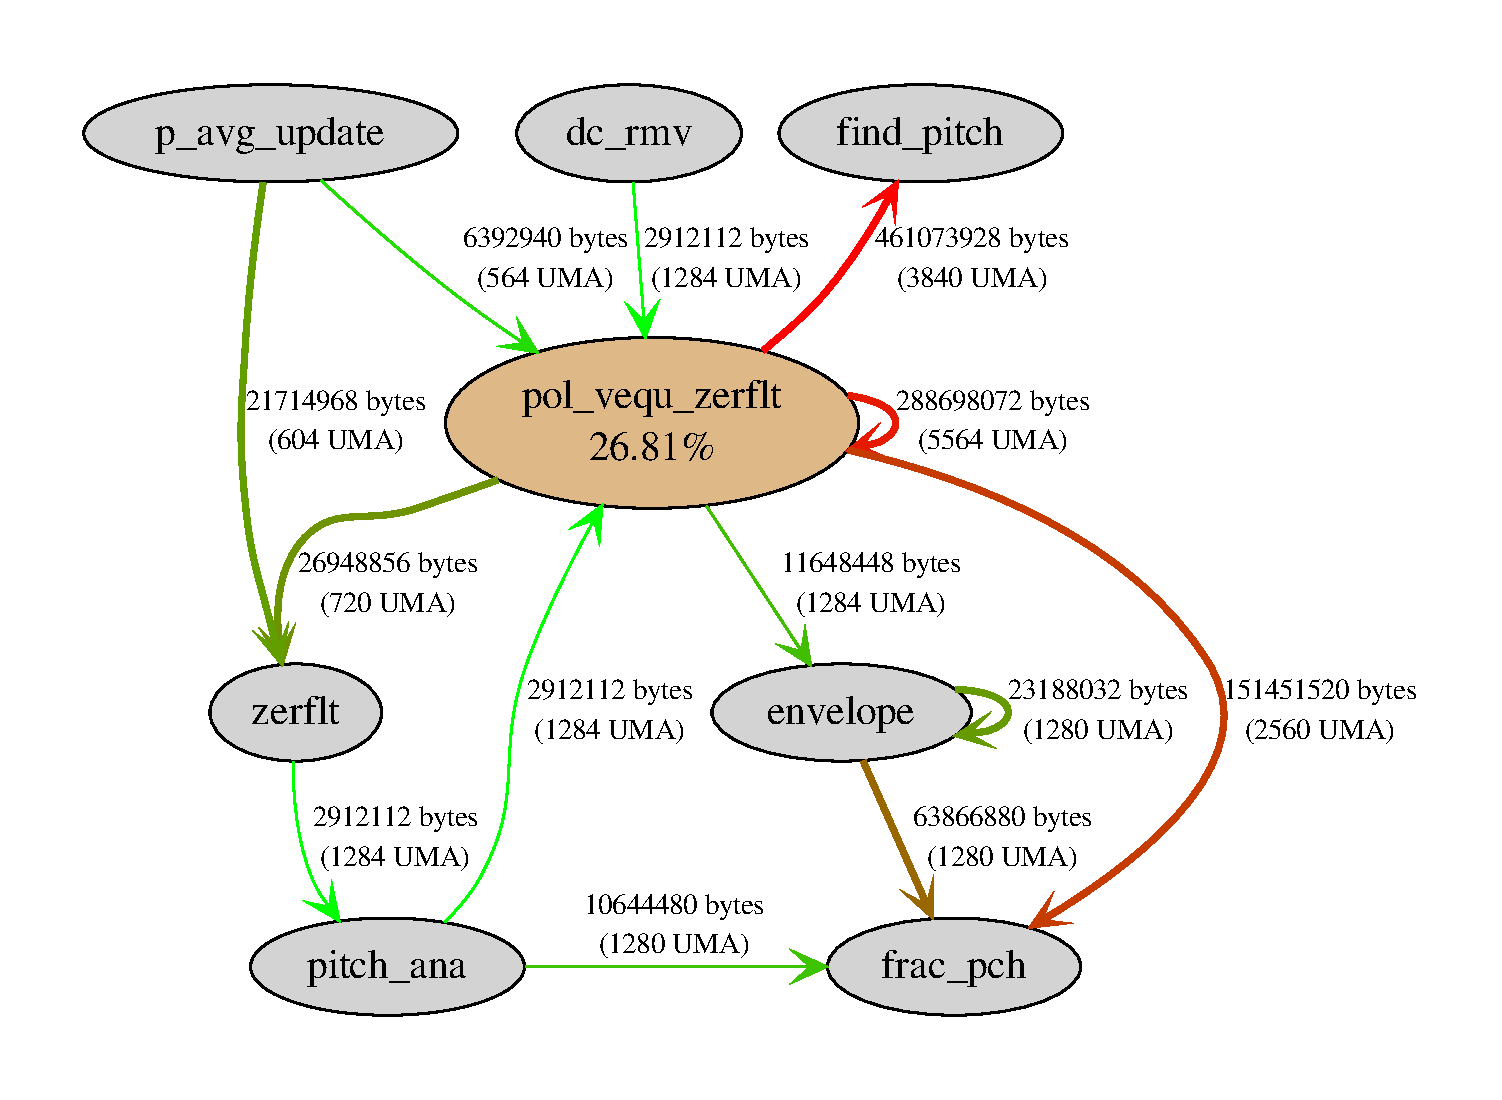
\includegraphics[width=0.67\linewidth]{figures/figure1.pdf}
% \caption{Figure 1 caption.}
% \label{fig:figure1}
% \end{figure}
% 
% 
% An example of an equation \ref{eq:amdhal}.
% \begin{equation}
% \label{eq:amdhal}
% \lim_{p \to \infty} \frac{p}{1-f(p-1)} = \frac{1}{f} = \frac{1}{1-s},
% \end{equation}
%  where $p$ is the speedup factor of the accelerated part, $f$ is the percentual
% contribution of the sequential part, and $s$ is the original percentual
% contribution of the accelerated part.

% \begin{figure} %[!bt]
% \centering
% \begin{verbatim}
% ReadImage-Byte2Float        9600
% Byte2Float-convolveHoriz    255360
% ComputeKernel-convolveVert  248640
% ComputeKernel-convolveHoriz 255360
% convolveHoriz-convolveVert  248640
% convolveVert-Float2Byte     38400
% Float2Byte-PrintImg         9600
% \end{verbatim}
% \caption{Simplified Output for the Image Convolution Application.}
% \label{fig:pincommout}
% \end{figure}
